% Section 5. Owners: 5.1 split; 5.2 each person for own algorithms; 5.3 text Abhishek; diagrams per docs/report/outline.md.
\section{Project Design}
\label{sec:design}

\subsection{Design Goals}
\label{sec:design-goals}

\paragraph{Heterogeneity, quality of service, scalability}
Volunteers differ in processor, memory and speed, and the coordinator cannot inspect them. Each volunteer therefore reports its CPU cores, memory and a speed score when it registers. Resource discovery uses the reported memory and speed (the cores are recorded but not used) together with a trust score learned from past votes: a volunteer that reports less than the configured minimum memory gets no units, a slow volunteer takes the newest units and leaves the end of a job to faster ones, and a volunteer with a poor record is kept away from deciding copies or blocked. Heterogeneity also threatens voting, since different processors can round floating-point operations differently. Rather than restrict votes to identical hardware, as BOINC's homogeneous redundancy does, we require every workload to return identical bytes on every architecture: the Monte Carlo workload uses only integer arithmetic, and the fractal workload rounds every product explicitly so that the compiler cannot fuse a multiply and an add on one architecture but not on another. Quality of service comes from bounding how long a unit can be held up. A lease bounds the wait for a lost unit to three minutes, and gossip usually shortens it to seconds; because a unit is accepted as soon as two of its three copies agree, one slow copy does not delay it. Scalability rests on two choices. Volunteers pull work, so the leader keeps no queue per volunteer and an idle volunteer costs one request per second, and gossip costs each member a constant number of messages per period, whatever the size of the group. Every table change still passes through the single leader, which is why the design targets units of about a minute: each unit then costs the leader only a few table changes (three assignments, up to three results and one acceptance) for several minutes of volunteer computation.

\paragraph{Openness}
All interaction happens through a single, versioned gRPC contract (Section~\ref{sec:components}). Any program that speaks this protocol can act as a client or a volunteer, and new workloads are added by implementing three functions (split, run, merge) without changing the coordinator. Every internal mechanism is a small Go interface with interchangeable implementations, so a team member can replace an algorithm without touching the rest of the system.

\paragraph{Security}
Volunteer computing gives work to machines that the operator does not control, so the coordinator must decide who may join and each volunteer must be able to tell a genuine task from a forged one. SpareCycles authenticates volunteers with per-volunteer tokens at registration and signs every task it hands out. A signature binds the task's payload to its unit, workload and lease expiry, so a captured task cannot be replayed for another unit or after its lease. Integrity of results, which a volunteer can still falsify, is protected separately by majority voting. Confidentiality of task data is out of scope (Section~\ref{sec:literature}).

\paragraph{Failure handling}
We treat failure as the normal case. A volunteer may stop at any moment; SWIM gossip declares it dead within seconds and the leader immediately releases its leases, while lease expiry remains as a slower safety net for volunteers that cannot take part in gossip. Every change to the task table is replicated before it takes effect, so a new leader can continue a job after the old one crashes. Faults are also contained: a volunteer that receives a task with a bad signature stops at once rather than taking more units it will never complete.

\paragraph{Concurrency, transparency}
A coordinator serves many volunteers and clients at the same time, and gRPC runs each request in its own goroutine, so all shared state must be guarded. The design keeps the number of possible orderings small. Every change to the task table passes through a single commit path that validates, replicates and applies it under one mutex, so the leader's changes form one total order, which is also the order in which the backups apply them. Recording a result and voting on its unit happen together under a second lock, so two results that arrive at the same moment yield one decision rather than two. The remaining shared state, such as the volunteer list, session hashes, trust scores and the election and gossip state, is protected by a mutex inside its own component, and the continuous integration pipeline runs every test with Go's race detector.

Transparency means that clients and volunteers never need to know which coordinator leads, or whether a failover has happened. They hold a connection to all three coordinators and send each call to the one that answered last. A follower answers \texttt{FAILED\_PRECONDITION} and a crashed node is \texttt{UNAVAILABLE}; in both cases the call moves on to the next coordinator (\texttt{leaderclient}). Replication is equally invisible: a job is confirmed only after its change is on two coordinators, so a client that polls a new leader finds its job where it left it. The only visible effect of a failover is that volunteers register again, because session secrets are deliberately kept on the leader alone.

\subsection{Key Components and Algorithms}
\label{sec:algorithms}

The system has three roles. \emph{Clients} submit jobs and fetch results. \emph{Coordinators}, three in total, hold the task table; one is the leader and the others are backups. \emph{Volunteers} pull work from the leader, run it and return results. Six algorithms from the course list work together:

\paragraph{Leases and reassignment (resource allocation)} When a volunteer pulls a unit, the leader records an assignment whose lease expires a fixed time later (\texttt{SC\_LEASE\_DURATION}, by default three minutes, three times the 60-second unit the design targets). The expiry is stored in the replicated task table and included in the signed task, and the volunteer cancels its own computation when the expiry passes. Once per second the leader asks the \texttt{lease.Timeout} policy for every lease in an open unit whose expiry has passed, and commits a \texttt{LeaseReleased} change for each; the unit then needs a volunteer again and goes to the next one that asks (Fig.~\ref{fig:unit-state}). A result is recorded only from a volunteer that still holds a lease on the unit, so a volunteer that lost its lease cannot complete the unit afterwards. Gossip normally frees the units of a crashed volunteer within seconds, well before the lease ends. The lease is the safety net for what gossip cannot see: a volunteer that runs with gossip turned off behind a home router, a volunteer that is alive but stuck, or a unit that takes far longer than planned.

\paragraph{Majority voting (agreement)} Each unit is sent to \texttt{SC\_VOTE\_REPLICAS} different volunteers, three by default, and the leader accepts an output once \texttt{SC\_VOTE\_QUORUM} results carry the same SHA-256 hash, two by default; the configuration rejects any quorum that is not a majority of the copies. The \texttt{verify.Majority} verifier runs after every recorded result, under a lock that makes recording and voting a single step, so a unit is accepted at the first moment two results agree, usually before its third copy returns. If every copy has returned and no output has a quorum, the leader raises the number of copies by two and sends the unit to two more volunteers, and repeats this until some output reaches the quorum. A volunteer never receives a unit for which it already holds a lease or has sent a result, so it contributes at most one result to each vote. Copies still running when a unit is accepted are not ignored: if such a copy returns before its lease ends, the leader compares it with the accepted output and counts it as wrong if it differs, as BOINC does for late results. Without this check, a faulty volunteer that always ran the third copy would never be caught (Section~\ref{sec:testing}).

\paragraph{Resource discovery} Volunteers report their CPU cores, memory and a speed score at registration (\texttt{SC\_CPU\_CORES}, \texttt{SC\_MEMORY\_MB}, \texttt{SC\_SPEED\_SCORE}). Because volunteers pull work, resource discovery decides which of the open units a requesting volunteer receives, or that it receives none. Building on VECTrust~\cite{pandey2021vectrust}, which models trust with a Dirichlet distribution, the leader keeps for each volunteer the two-outcome special case, a beta reputation $(c+1)/(c+w+2)$, where $c$ and $w$ count the volunteer's results that agreed and disagreed with an accepted output; a new volunteer starts at 0.5. The \texttt{scheduler.Matcher} applies five rules in order. A volunteer that reports less memory than \texttt{SC\_MIN\_MEMORY\_MB} gets nothing. A volunteer whose trust falls below \texttt{SC\_TRUST\_MIN} (0.3) is blocked for good, which for a new volunteer happens at its second wrong result (trust 0.25). A volunteer below \texttt{SC\_TRUST\_LAST\_COPY} (0.6) skips units where it would take the last copy, since that copy often decides the vote, unless no other unit is available. A volunteer whose speed score is below \texttt{SC\_SLOW\_SPEED} (0.5) takes the newest unit instead of the oldest while a fast volunteer is active, and gets nothing at the end of the work when the active fast volunteers can take every open copy themselves. Every other request receives the oldest unit. A fast volunteer counts as active for one lease length after its last request, or until gossip declares it dead.

\paragraph{Leader election} The three coordinators run the Bully algorithm~\cite{garciamolina1982elections} extended with terms and a leader lease. The leader sends a heartbeat every \texttt{SC\_ELECTION\_HEARTBEAT} (500\,ms). A follower that hears no leader for \texttt{SC\_ELECTION\_TIMEOUT} (2\,s), plus a random delay of up to a quarter of it, increments its term and sends an election message to every node with a higher identifier. If none answers, it announces itself, and it wins only if a majority (2 of 3, counting itself) accepts it. A node accepts at most one leader per term, and it answers a message from an older term with its own newer term, which makes the sender step down. A node also refuses a new leader within one lease of answering another, and a winner waits one lease after it last answered the previous leader, so the old leader's lease has ended before the new one acts. Before acting, the winner also loads the newest task table (see below). The leader acts only while a majority has answered a heartbeat within the lease of \texttt{SC\_ELECTION\_TIMEOUT} minus \texttt{SC\_ELECTION\_HEARTBEAT} (1.5\,s), counted from when the heartbeat was sent; otherwise it steps down. A follower that receives a heartbeat from a lower node starts an election to take over, so the highest live node eventually leads. A node that still hears a live leader answers election messages but does not start an election itself, so an isolated node cannot disturb a working leader.

\paragraph{Replication and consistency} The task table is replicated in a primary-backup scheme. Each change carries a log index, one more than the index of the leader's table. The leader validates the change, sends it to both backups in parallel, and applies it only after one backup has applied it, so every confirmed change exists on 2 of 3 coordinators; the other backup receives it in the background. If no backup confirms within \texttt{SC\_REPLICATION\_TIMEOUT} (1\,s), the leader drops the change, and the caller receives \texttt{UNAVAILABLE} and retries. A backup rejects changes from an older term, applies changes strictly in index order, and treats a repeated index with the same content as a retry. When it sees a gap, a different change at its last index, or the first change of a new term, it loads a full snapshot of the leader's table instead; this also discards any change that an old leader sent but never confirmed. Because Bully elects the highest identifier rather than the most up-to-date node, a new leader first asks every reachable coordinator for its snapshot and adopts the one with the highest index (\emph{catch-up}). The volunteer list, session secrets, trust scores and late-copy records are deliberately not replicated; after a failover, volunteers register again.

\paragraph{Gossip-based failure detection}
Coordinators and volunteers form a single SWIM group. Each member probes one other member per period in shuffled round-robin order, falls back to $k$ indirect probes when a direct probe fails, and marks an unresponsive member suspect and later dead (Fig.~\ref{fig:swim-state}). Every message carries the sender's own record and up to eight recent updates, each of which is forwarded about $3\lceil\log_2 n\rceil$ times. The coordinators seed the group with each other, and the leader adds each volunteer when it registers; the volunteer then learns the rest of the group from the leader's first probe. Once a volunteer is declared dead, the leader releases its leases and forgets it, so its units move on before their leases expire.

\paragraph{Authentication and signed tasks}
At registration the leader compares the volunteer's token with a list of named tokens, in constant time over all entries so that response time reveals nothing about near matches. A successful registration returns the volunteer's identifier together with a random session secret, which the volunteer attaches to every later request; the leader stores only the secret's hash and rejects any request whose secret does not match. For each task, the leader signs a message with Ed25519~\cite{bernstein2012ed25519} that encodes a domain tag, the unit identifier, the workload name, the lease expiry and the payload, with a length prefix on every variable-length field and the lease expiry as a fixed eight-byte field. The volunteer rebuilds the same message and verifies the signature before it runs any code.

\begin{figure}[t]
\centering
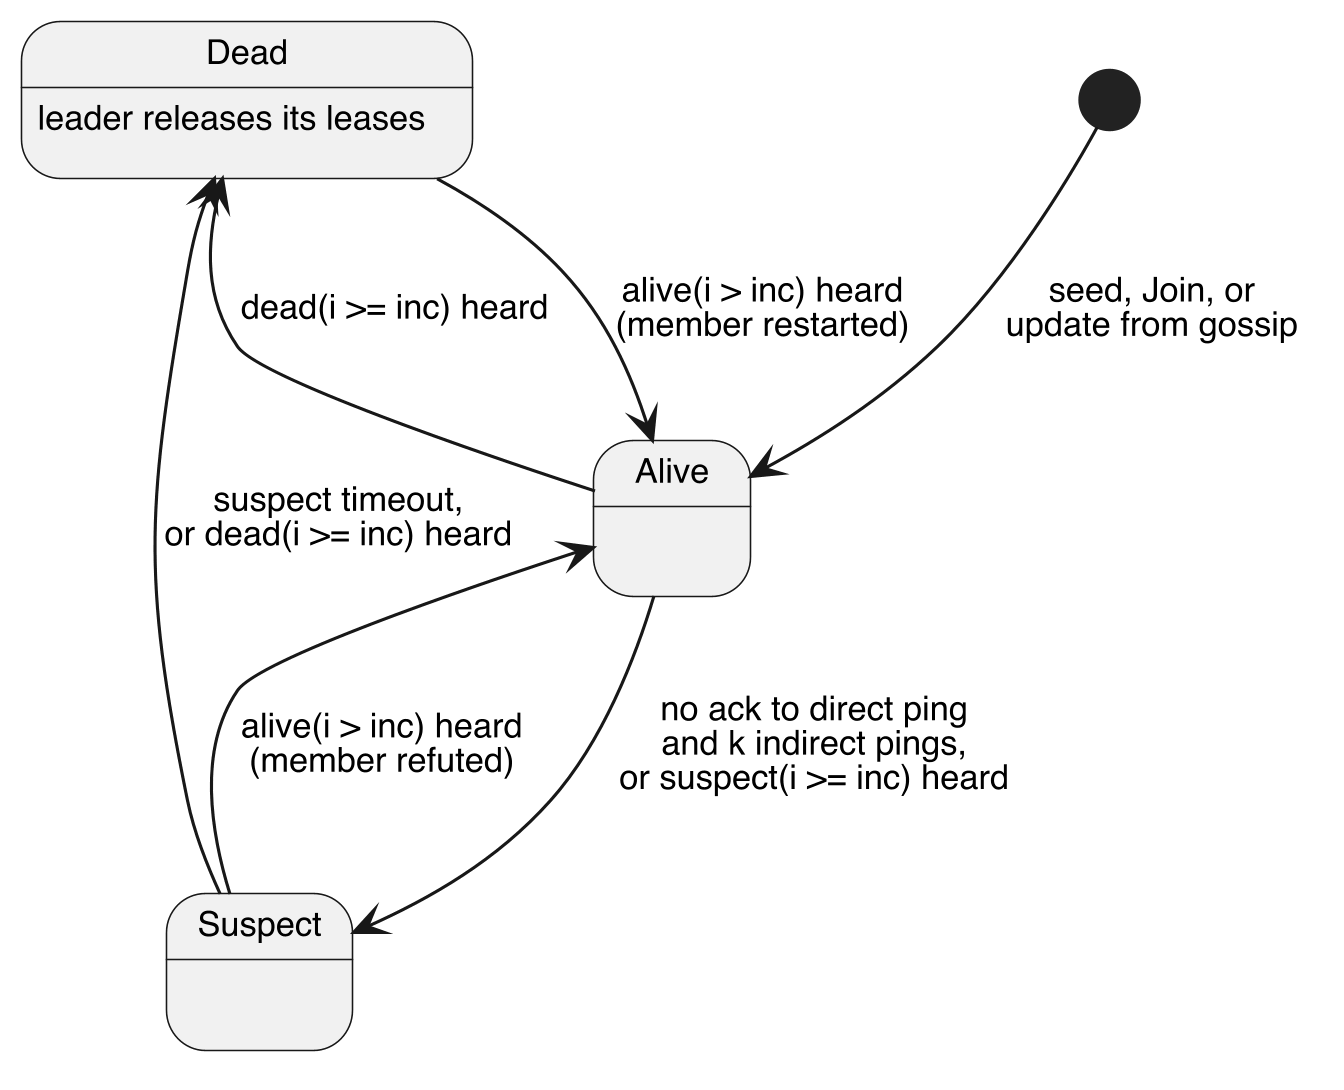
\includegraphics[width=0.9\columnwidth]{d6-swim-state.png}
\caption{What one SWIM member believes about another (design diagram D6). Updates carry an incarnation number $i$; \textit{inc} is the incarnation currently known for the member.}
\label{fig:swim-state}
\end{figure}

\subsection{Architecture}
\label{sec:architecture}

Fig.~\ref{fig:use-case} summarizes what each actor can do. A \emph{client} submits a job, follows its progress and retrieves the merged result. A \emph{volunteer} registers with its token and its resources, requests work and returns results. An \emph{operator} starts and stops the cluster, sets tokens, keys and timeouts, and watches the metrics.

Fig.~\ref{fig:deployment} shows the target deployment. Three coordinators run in three AWS availability zones, so that the loss of one zone still leaves a majority. Volunteers run on EC2 spot instances spread over the zones and on the team's laptops, and a Prometheus server scrapes the metrics of every coordinator. Each process is a single Go binary configured by environment variables, so the same topology also runs as local processes or with Docker Compose. Terraform files create the AWS deployment; all measurements in this report were taken on one machine.

The components interact over the five gRPC services of Section~\ref{sec:components}. Clients and volunteers talk only to the leader, and work always flows by pull: the leader opens connections to volunteers only for gossip probes. The coordinators talk to each other for election and replication, and all coordinators and volunteers form one SWIM group (Fig.~\ref{fig:swim-state}). Inside the leader, the coordinator server is the only component that changes the task table. It consults the scheduler for resource discovery, the lease policy, the verifier for voting and the membership view, and sends each resulting change through replication.

Each unit moves through the states of Fig.~\ref{fig:unit-state}. A unit is open while it still needs copies; each copy is leased to a different volunteer, whose result is then recorded; and the unit is accepted when two results agree. If every copy is back and no two agree, the leader asks for two more copies and the unit needs volunteers again. A lease that expires, or whose volunteer gossip declares dead, returns its copy without a result. Fig.~\ref{fig:failover} shows a leader crash: heartbeats stop, the highest remaining coordinator starts an election in a new term, wins with the acceptance of the third coordinator, catches up to the newest table and starts serving. Clients and volunteers find it by moving past the unreachable old leader and the follower that answers \texttt{FAILED\_PRECONDITION}, and volunteers then register again.

\begin{figure}[t]
  \centering
  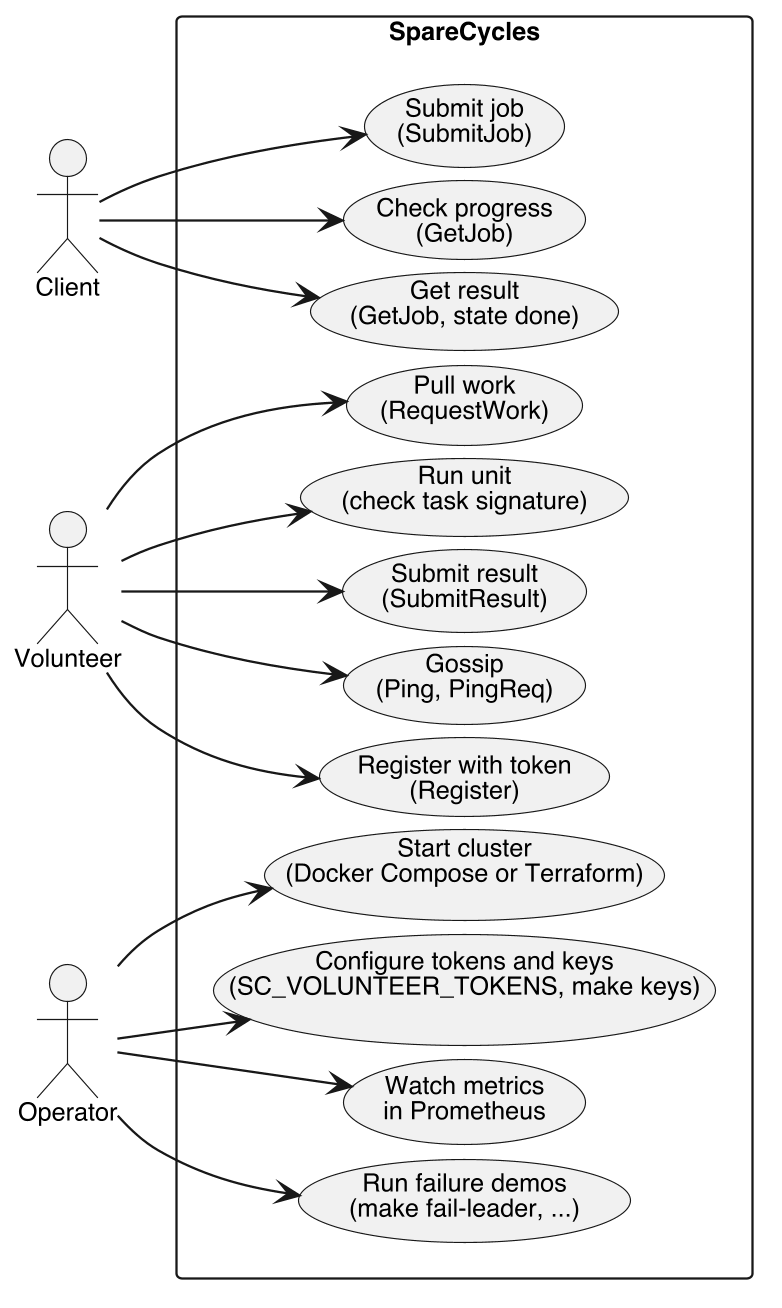
\includegraphics[width=0.8\columnwidth]{d1-use-case.png}
  \caption{Use cases of the three actors (design diagram D1). Clients and volunteers interact with the system only through gRPC calls to the leader and SWIM gossip, while the operator works outside the protocol through deployment, configuration, monitoring and the scripted failure demos.}
  \label{fig:use-case}
\end{figure}

\begin{figure*}[t]
  \centering
  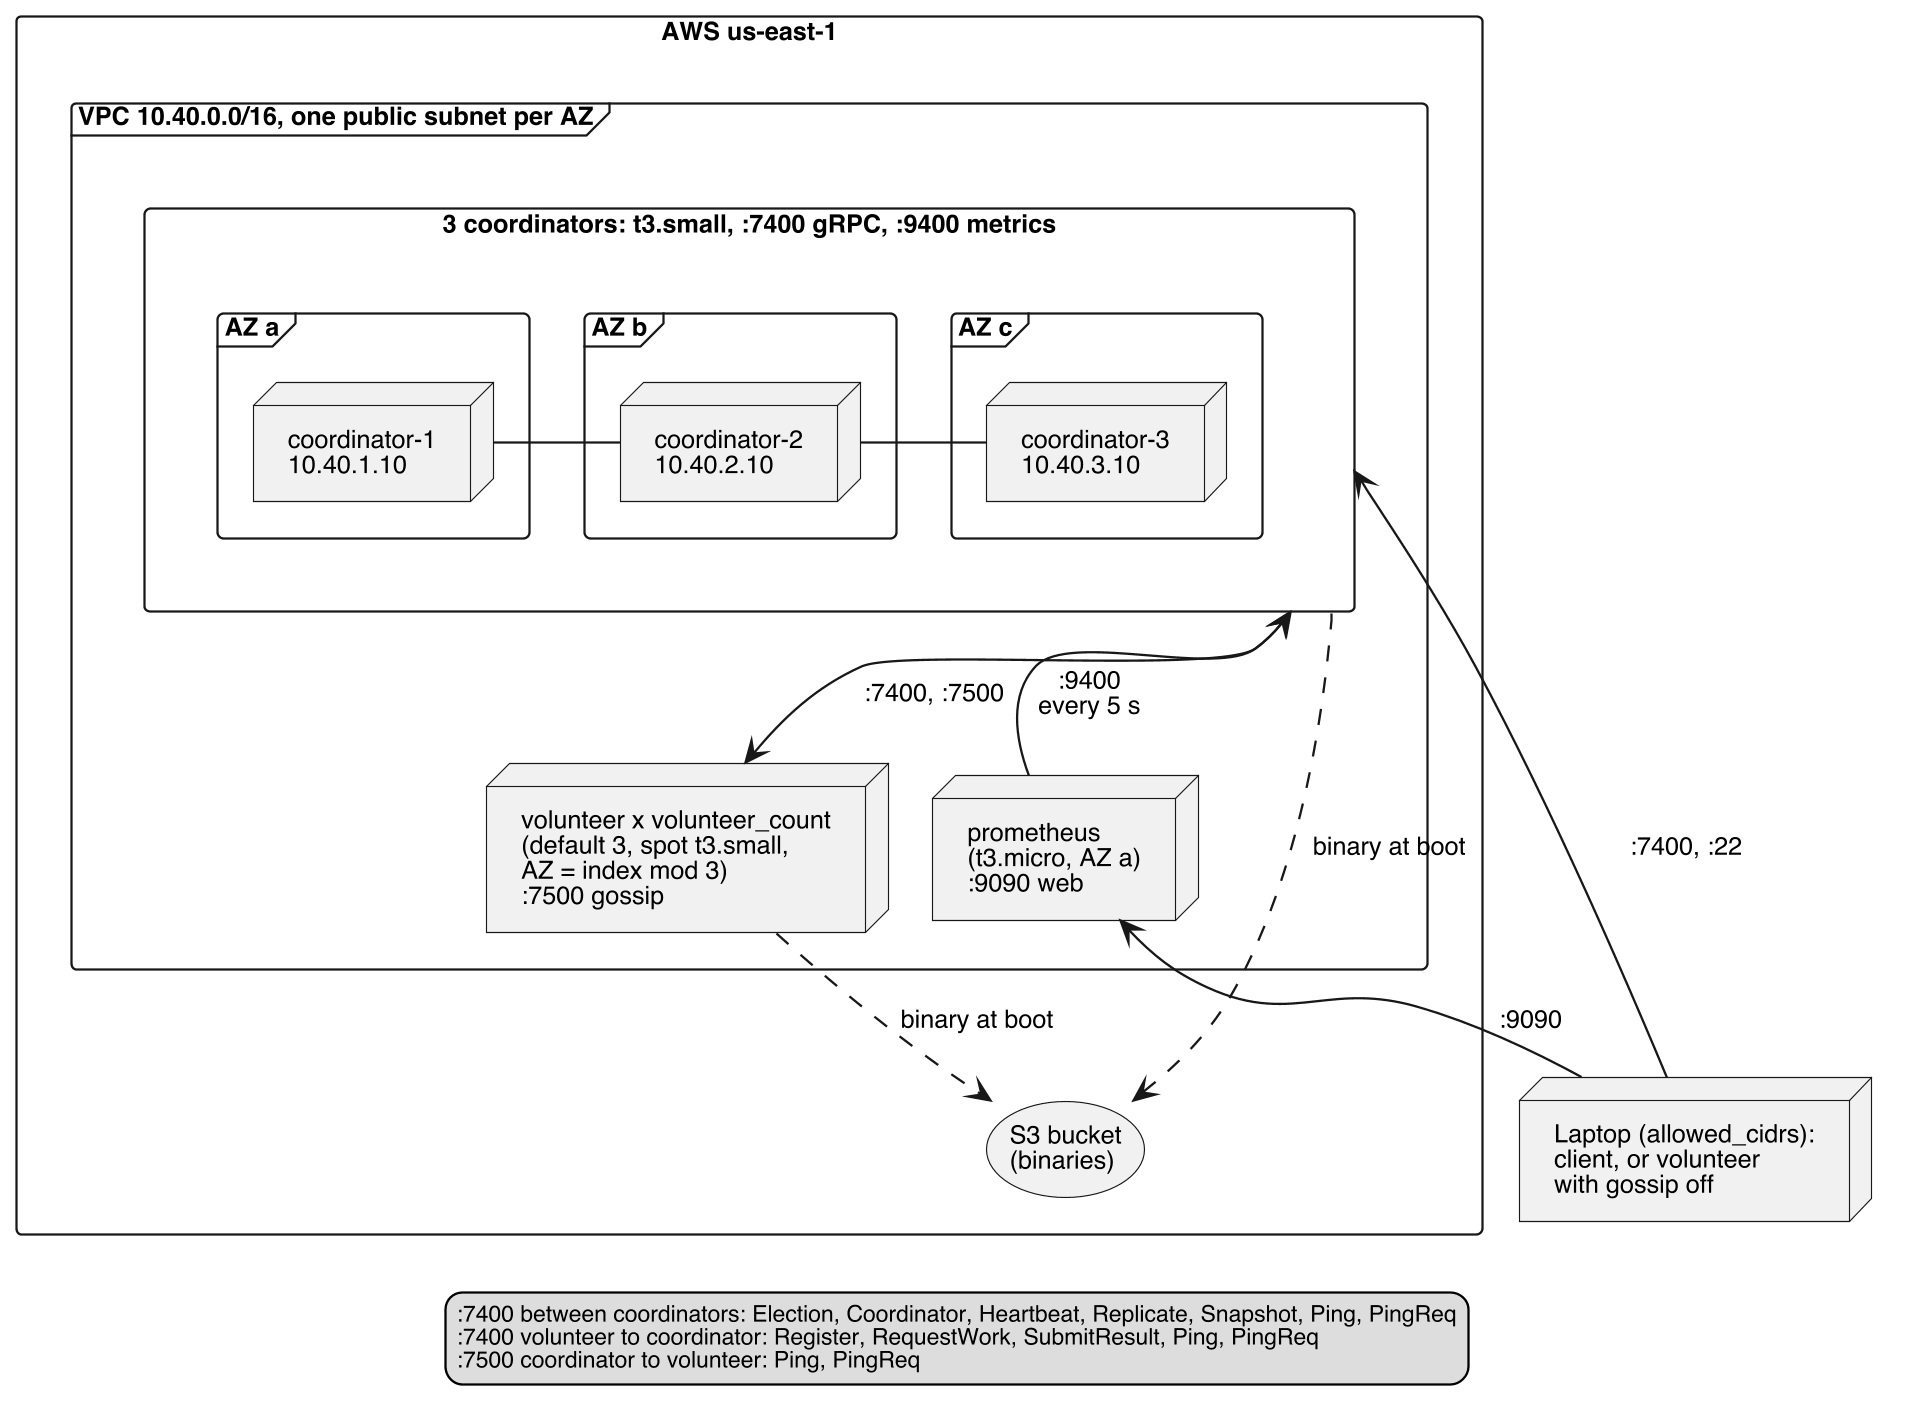
\includegraphics[width=0.78\textwidth]{d2-deployment.png}
  \caption{AWS deployment created by the Terraform configuration (design diagram D2). The three coordinators sit in separate availability zones with fixed private addresses, so the loss of one zone leaves a two-of-three majority, and the volunteers run on spot instances whose interruptions the lease and gossip mechanisms absorb.}
  \label{fig:deployment}
\end{figure*}

\begin{figure}[t]
  \centering
  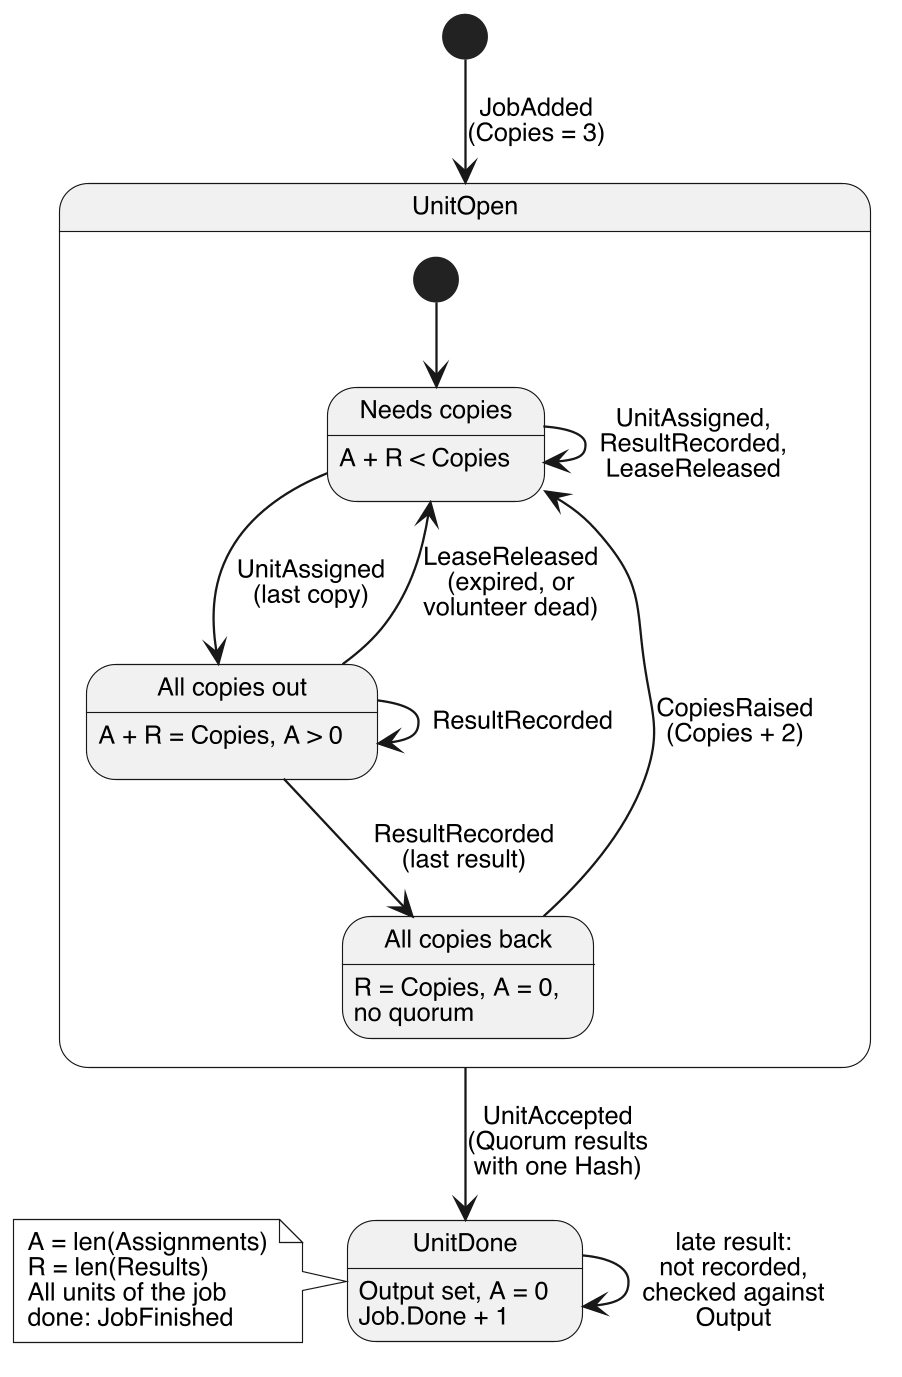
\includegraphics[width=0.85\columnwidth]{d4-unit-state.png}
  \caption{Life cycle of one work unit in the task table (design diagram D4). Each transition is a replicated task-table change; the table itself stores only \texttt{UnitOpen} and \texttt{UnitDone}, and the sub-states of an open unit follow from its number of leases and results.}
  \label{fig:unit-state}
\end{figure}

\begin{figure}[t]
  \centering
  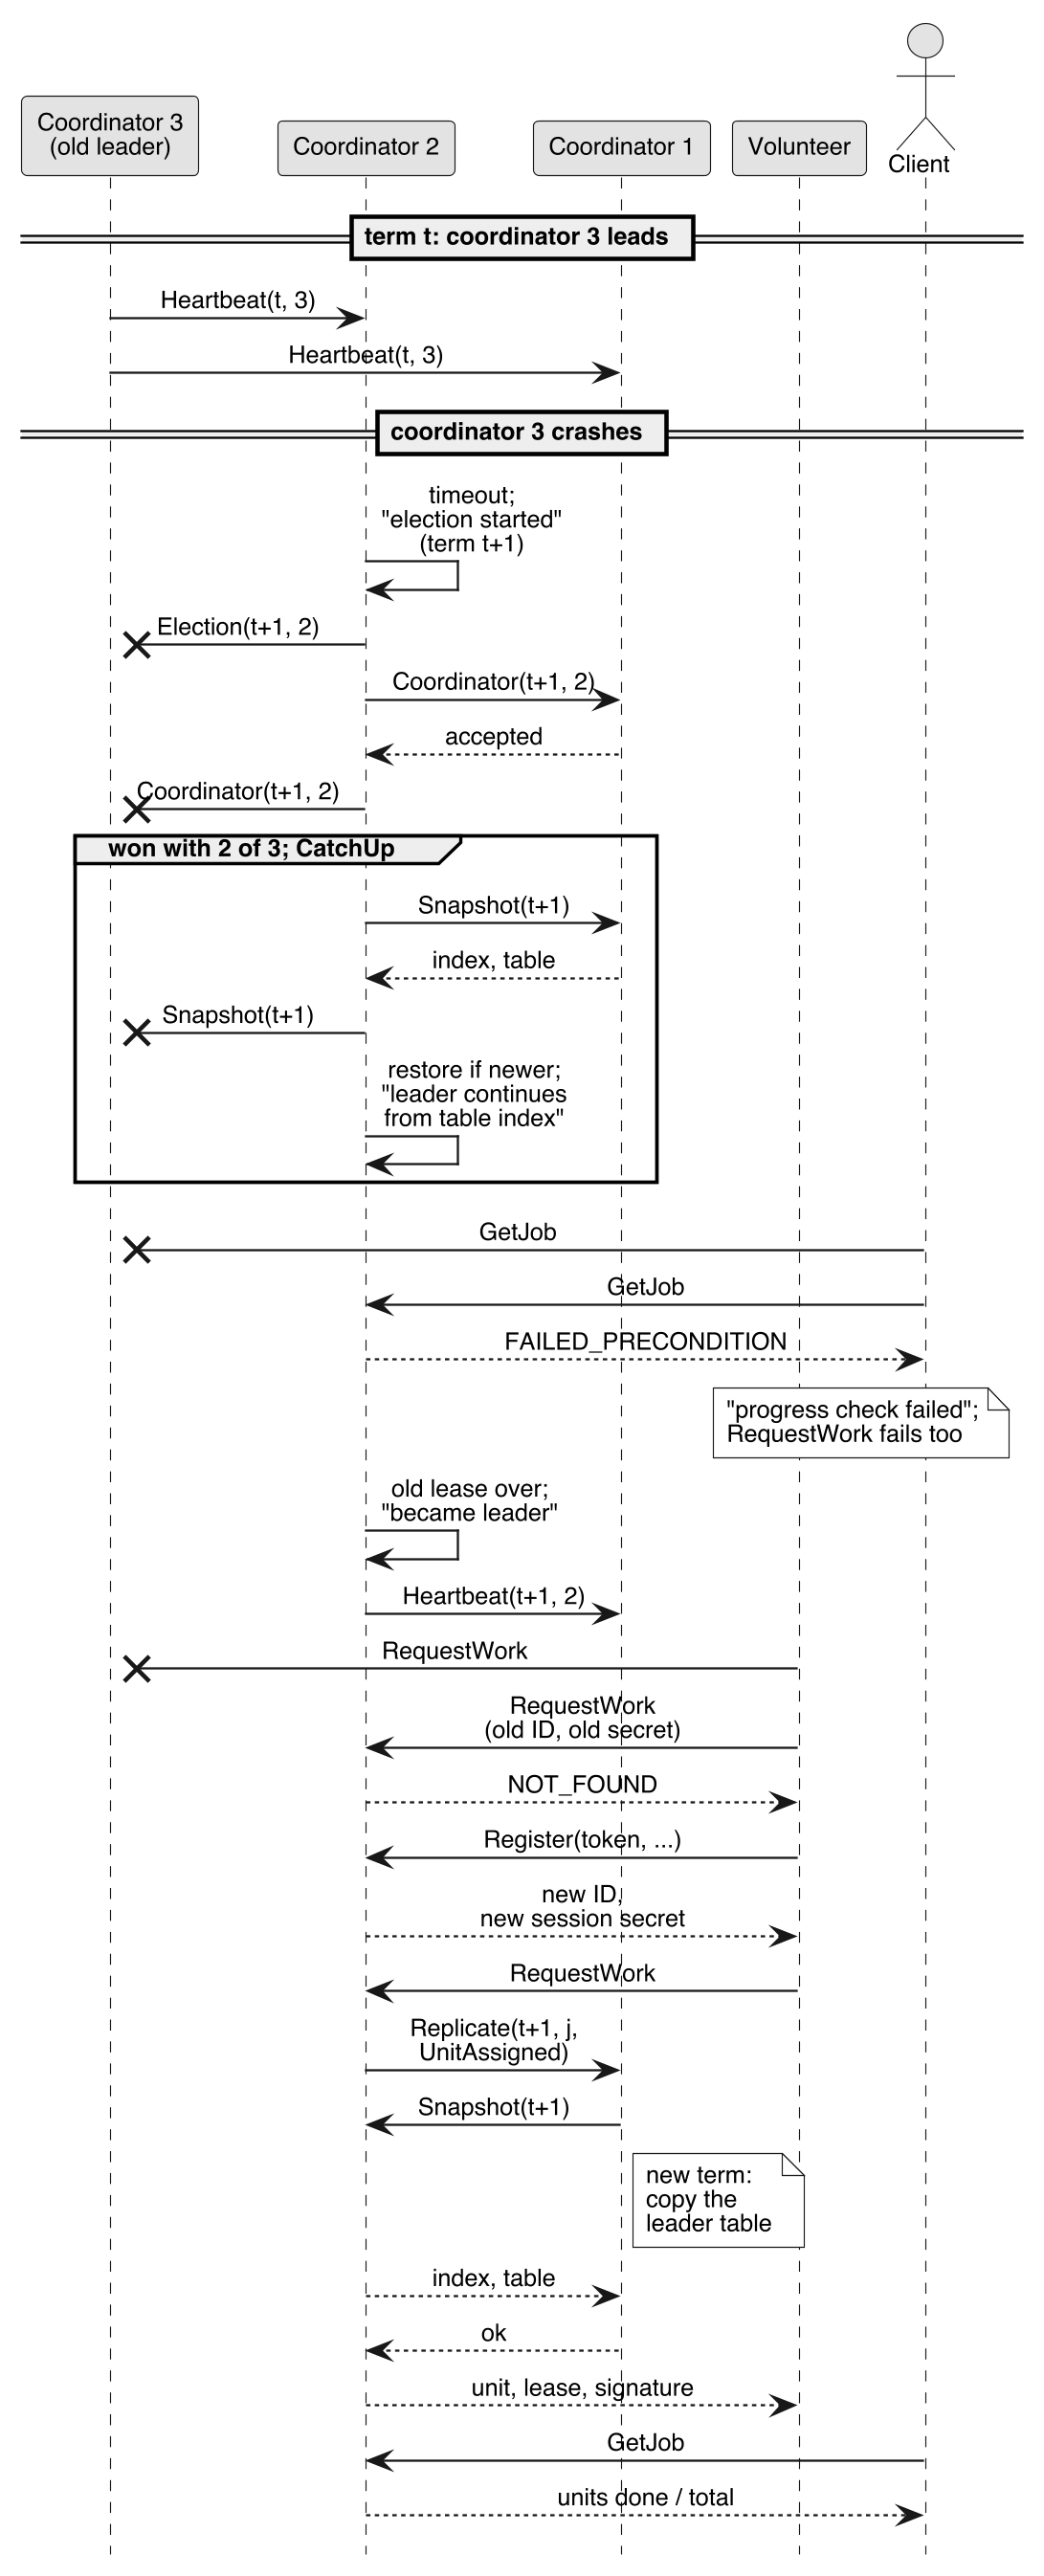
\includegraphics[width=0.72\columnwidth]{d5-failover-sequence.png}
  \caption{Failover after a crash of the leader (design diagram D5). Coordinator 2 wins a higher term with a majority, loads the newest table from the reachable coordinators before it acts, and the volunteer registers again because volunteer sessions are not replicated.}
  \label{fig:failover}
\end{figure}

Figure~\ref{fig:job-sequence} shows the life of one job. The leader splits the job into units and replicates the change before it confirms the job to the client. Volunteers pull units; each unit is given to three different volunteers, each with a lease and a signature. When two results agree, the leader accepts the unit, and when every unit is accepted it merges the outputs and records the final result.

\begin{figure*}[t]
\centering
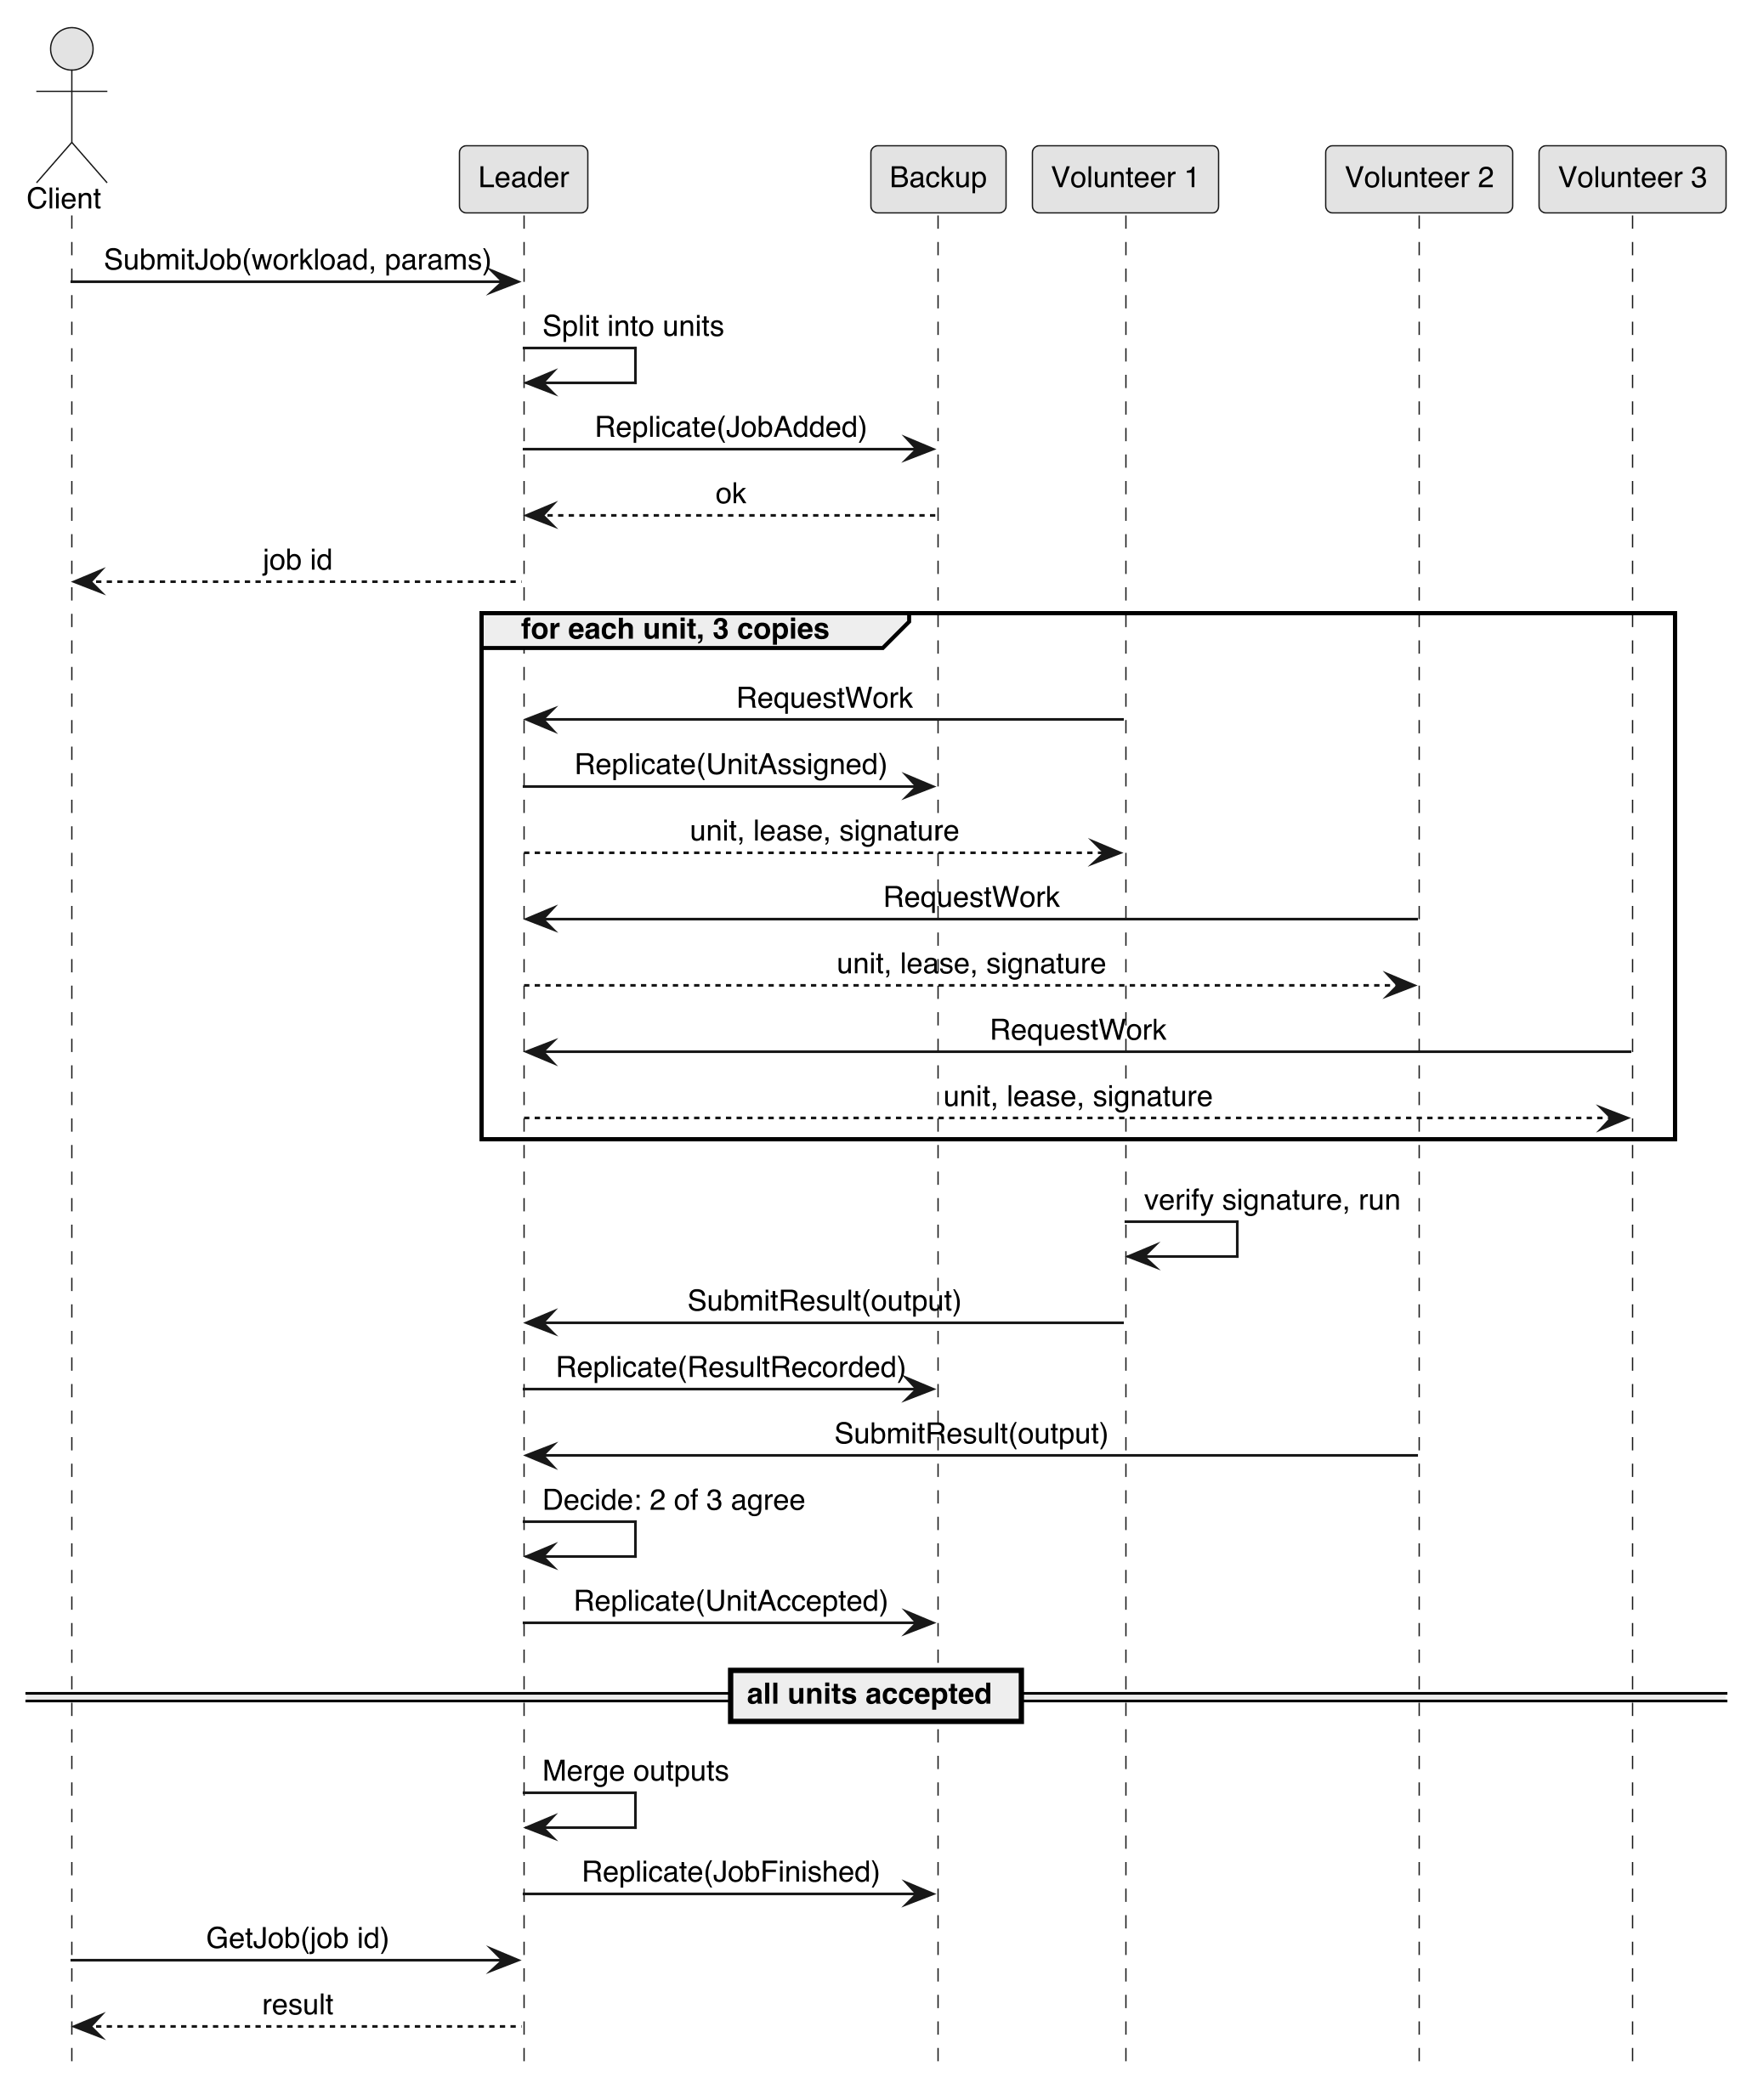
\includegraphics[width=0.8\textwidth]{d3-job-sequence.png}
\caption{One job from submission to result (design diagram D3). Every change to the task table is replicated to a backup before it is applied.}
\label{fig:job-sequence}
\end{figure*}
